\documentclass[tikz,border=10pt]{standalone}
\usetikzlibrary{angles}
\begin{document}
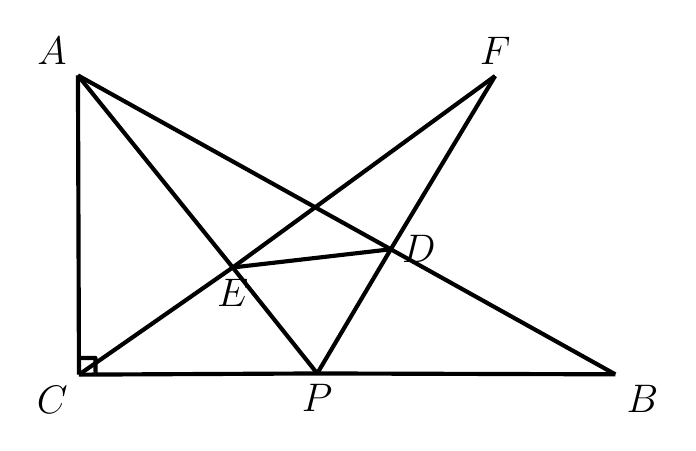
\begin{tikzpicture}[line width=1.5pt, line join=round]
\coordinate (A) at (-3.432,1.902);
\coordinate (B) at (3.392,-1.894);
\coordinate (C) at (-3.419,-1.898);
\coordinate (D) at (0.541,-0.306);
\coordinate (E) at (-1.466,-0.537);
\coordinate (F) at (1.866,1.895);
\coordinate (O) at (1.170,-0.656);
\coordinate (P) at (-0.393,-1.883);











  
  \draw (A) -- (C);
  \draw (C) -- (P) -- (B);
  \draw (A) -- (D) -- (B);
  \draw (A) -- (E) -- (P);
  \draw (C) -- (E) -- (F);
  \draw (F) -- (D) -- (P);
  \draw (D) -- (E);

  
  \draw pic[draw, line width=1.5pt, angle radius=0.211cm] {right angle=B--C--A};

  
  \node[above left]  at (A) {\fontsize{15}{18}\selectfont $A$};
  \node[below left]  at (C) {\fontsize{15}{18}\selectfont $C$};
  \node[below right] at (B) {\fontsize{15}{18}\selectfont $B$};
  \node[below]       at (P) {\fontsize{15}{18}\selectfont $P$};
  \node[above]       at (F) {\fontsize{15}{18}\selectfont $F$};
  \node[below]       at (E) {\fontsize{15}{18}\selectfont $E$};
  \node[right]       at (D) {\fontsize{15}{18}\selectfont $D$};
\end{tikzpicture}
\end{document}